
\chapter{Masterframe}
\label{cha:masterframe}

In dit hoofdstuk zal er een masterframe opgebouwd worden zoals beschreven in \cite{Tessema}. Vooraf moet er nagedacht worden over wat de robot allemaal kan en hoe die dan zou aangestuurd kunnen worden door een gebruiker. Uit deze lijst van mogelijke spraakcommando's (komende uit de natuurlijke taal) zal dan een masterframe opgesteld worden zodat de commando's hierarchisch gestructureerd worden. De robot is te zien in Figuur ~\ref{fig:robot}. Deze kan vooruit en achteruit rijden, draaien en met de grijper vooraan kan hij objecten oppakken. Bovendien heeft de robot een aantal sensoren om objecten te detecteren en om aan tracking te doen. \\

\begin{figure}[h]
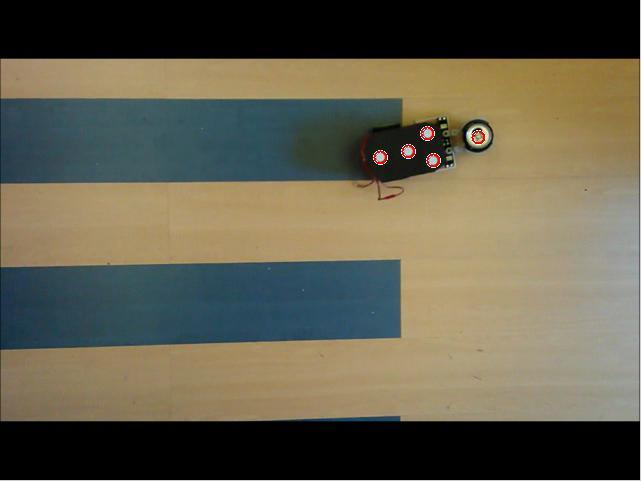
\includegraphics[width=0.5\textwidth]{robot.jpg}
\label{fig:robot}
\centering
\caption{Foto van de gebruikte robot}
\end{figure}

\section{Frames}
\label{sec:frames}

De eenvoudigste opdrachten die een gebruiker de robot zou kunnen geven is om te bewegen. Enkele voorbeelden hiervan zijn '\textit{ga naar daar}' of '\textit{rij 5cm vooruit}'. Er wordt hier onderscheid gemaakt tussen drie soorten bewegingen:

\begin{itemize}
\item een absolute beweging: dit is een beweging naar een vast punt in het frame zoals bv. de hoek of het midden. Dit zou ook een object kunnen zijn.
\item een relatieve beweging: dit is een beweging relatief ten opzichte van zijn huidige positie zoals een bepaalde afstand voorruit of naar links rijden. 
\item bewegen voor een bepaalde tijd: dit kan zijn tot de gebruiker stop zegt of voor een bepaalde tijdsduur.
\end{itemize}

Elke soort van de opgesomde bewegingen kan een rotatie en/of een translatie bevatten.  \\
\\
Andere commando's zijn commando's waarvoor de robot zijn grijper nodig heeft. Dit zouden eenvoudige dingen kunnen zijn zoals '\textit{grijp}' of '\textit{laat los}'. Voor deze commando's moet de robot maar \'e\'en actie uitvoeren, namelijk zijn grijper sluiten of openen. Er zijn echter ook complexere commando's zoals '\textit{breng het blikje naar de bal}'. Hiervoor moet de robot verschillende dingen doen; hij moet het blikje vinden, naar het blikje rijden, het blikje pakken, de bal vinden, naar de bal rijden en zijn grijpers openen om het blikje los te laten.\\
\\
Uit de bovenstaande beschrijving wordt er een mogelijke lijst van commando's gehaald. Dit zijn de frames in onze masterframe. Deze zijn te zien in tabel \ref{tab:commands}.

\begin{table}[h]
\centering
\begin{tabular}{| l | l |}
\hline
\textbf{move\_rel} &  bewegen relatief ten opzichte van de huidige positie\\
\textbf{move\_abs} & bewegen naar een vast punt in het frame\\
\textbf{move\_to\_obj} & bewegen naar een object\\
\textbf{move\_time} & bewegen voor een bepaalde tijd\\
\textbf{turn\_abs} & zich richten naar een bepaalde richting\\
\textbf{turn\_rel} & een bepaalde hoek draaien relatief ten opzichte van de huidige ori"entatie\\
\textbf{turn\_time} & draaien voor een bepaalde tijd\\
\textbf{grab} & grijpen met de grijpers\\
\textbf{release} & de grijpers openen\\
\textbf{grab\_obj} & een bepaald object pakken\\
\textbf{move\_obj} & een object verplaatsen naar een andere locatie\\
\textbf{stop} & stop de huidige actie\\
\hline
\end{tabular}
\caption{Lijst van commando's}
\label{tab:commands}
\end{table}

\section{Slots en slotvalues}
\label{sec:slots_slotvalues}

Voor alle commando's die opgesomd zijn in tabel \ref{tab:commands} moet er beslist worden welke parameters er moeten worden meegegeven met de commando's en welke waardes deze kunnen aannemen. De parameters worden de slots genoemd en de bijhorende waarden de slotvalues. Bij de keuze van deze parameters (en bijhorende waarden) is er rekening gehouden met de verwachte input. De commando's zouden immers op een zo natuurlijk mogelijke manier moeten kunnen gegeven worden. Een normale gebruiker zal bijvoorbeeld zelden zeggen: '\textit{rij naar positie met x-co"ordinaat 3 en y-co"ordinaat 5}' maar zal eerder iets zeggen als '\textit{rij naar het midden}'. Achteraf zal dit midden in het verdere programma wel co"ordinaten krijgen, maar dit heeft geen invloed voor de gebruiker.\\
\\
Voor de afstanden die de robot relatief ten opzichte van zijn huidige positie kan afleggen wordt er gekozen voor een exponentieel (of hi"erarchisch) verloop omdat voor kleine bewegingen van de robot een hogere precisie nodig is dan voor grotere bewegingen.\\
De robot kan ook bewegen naar vaste punten. Zoals al vermeld moeten deze punten benoembaar zijn in de natuurlijke taal e.g. 'het midden'. Daarom wordt voor de vaste posities gekozen voor het midden, de hoeken en het midden van de wanden. Deze plaatsen zullen benoemd worden zoals de windrichtingen zoals in Figuur ~\ref{fig:masterframe}.\\
Voor de acties waarbij de robot moet bewegen voor een bepaalde tijd moeten er verschillende duraties zijn, maar het moet ook mogelijk zijn om de robot te laten bewegen tot de gebruiker stop zegt (de rotatie kan zo bv gebruikt worden om de robot te richten). In dit laatste geval is het echter wel prefereerbaar om te robot traag te laten bewegen zodat deze niet te lang blijft door roteren door de inherente vertraging van de spraaksoftware. De tijden worden net zoals de afstanden exponentieel gekozen.\\
De hoeken die de robot moet kunnen draaien, moeten alsook in de natuurlijke taal benoemd kunnen worden. Logische keuze's zijn alvast $90^\circ$ en $180^\circ$ voor bv. 'draai naar links' of 'draai om'. $45^\circ$ is ook nog gekozen voor bv 'draai schuin naar rechts'.\\
Het absoluut richten van de robot moet mogelijk zijn naar alle 'windrichtingen'. De hoeken zijn dus gekozen van $0^\circ$ tot en met $315^\circ$ in stappen van $45^\circ$. Deze absolute hoeken worden gemeten ten opzichte van bv. de onderste plank van het frame waarin de robot beweegt.\\
\\
Met al deze gemaakte beslissingen kan nu het masterframe opgesteld worden. Deze is te zien in Figuur \ref{fig:masterframe}. De tijden worden hierin weergegeven in seconden en de afstanden in centimeter omdat met de huidige opstelling dit de meest waarschijnlijke dimensies zijn die uitgesproken zullen worden.

\begin{figure}[h]
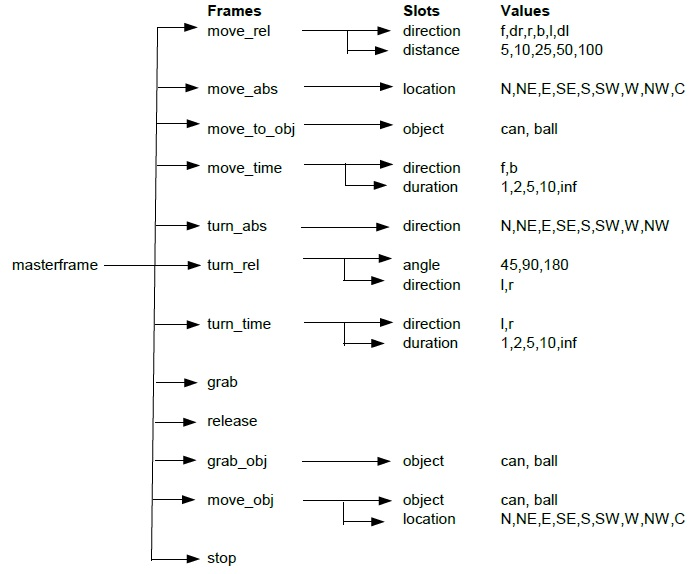
\includegraphics[width=\textwidth]{masterframe.jpg}
\label{fig:masterframe}
\centering
\caption{Het gekozen masterframe}
\end{figure}
